\documentclass[12pt]{article}
\usepackage[margin=1in]{geometry}
\usepackage{setspace}
\onehalfspacing{}
\usepackage[dvipsnames,table,xcdraw]{xcolor} % colors

% Start of preamble
%==========================================================================================%
% Required to support mathematical unicode
\usepackage[warnunknown, fasterrors, mathletters]{ucs}
\usepackage[utf8x]{inputenc}

% Standard mathematical typesetting packages
\usepackage{amsmath,amssymb,amscd,amsthm,amsxtra, pxfonts}
\usepackage{mathtools,mathrsfs,xparse}

% Symbol and utility packages
\usepackage{cancel, textcomp}
\usepackage[mathscr]{euscript}
\usepackage[nointegrals]{wasysym}
\usepackage{apacite}

% Extras
\usepackage{physics}  % Lots of useful shortcuts and macros
\usepackage{tikz-cd}  % For drawing commutative diagrams easily
\usepackage{microtype}  % Minature font tweaks
%\usepackage{pgfplots} % plots

\usepackage{enumitem}
\usepackage{titling}

\usepackage{graphicx}

%\usepackage{quiver}

% Fancy theorems due to @intuitively on discord
\usepackage{mdframed}
\newmdtheoremenv[
backgroundcolor=NavyBlue!30,
linewidth=2pt,
linecolor=NavyBlue,
topline=false,
bottomline=false,
rightline=false,
innertopmargin=10pt,
innerbottommargin=10pt,
innerrightmargin=10pt,
innerleftmargin=10pt,
skipabove=\baselineskip,
skipbelow=\baselineskip]{mytheorem}{Theorem}

\newenvironment{theorem}{\begin{mytheorem}}{\end{mytheorem}}

\newtheorem{corollary}{Corollary}
\newtheorem{lemma}{Lemma}

\newtheoremstyle{definitionstyle}
{\topsep}%
{\topsep}%
{}%
{}%
{\bfseries}%
{.}%
{.5em}%
{}%
\theoremstyle{definitionstyle}
\newmdtheoremenv[
backgroundcolor=Violet!30,
linewidth=2pt,
linecolor=Violet,
topline=false,
bottomline=false,
rightline=false,
innertopmargin=10pt,
innerbottommargin=10pt,
innerrightmargin=10pt,
innerleftmargin=10pt,
skipabove=\baselineskip,
skipbelow=\baselineskip,
]{mydef}{Definition}
\newenvironment{definition}{\begin{mydef}}{\end{mydef}}

\newtheorem*{remark}{Remark}

\newtheorem*{example}{Example}
\newtheorem*{claim}{Claim}

% Common shortcuts
\def\mbb#1{\mathbb{#1}}
\def\mfk#1{\mathfrak{#1}}

\def\bN{\mbb{N}}
\def\C{\mbb{C}}
\def\R{\mbb{R}}
\def\bQ{\mbb{Q}}
\def\bZ{\mbb{Z}}
\def\cph{\varphi}
\renewcommand{\th}{\theta}
\def\ve{\varepsilon}
\newcommand{\mg}[1]{\| #1 \|}

% Often helpful macros
\newcommand{\floor}[1]{\left\lfloor#1\right\rfloor}
\newcommand{\ceil}[1]{\left\lceil#1\right\rceil}
\renewcommand{\qed}{\hfill\qedsymbol}
\renewcommand{\ip}[1]{\langle#1\rangle}
\newcommand{\seq}[2]{\qty(#1_#2)_{#2=1}^{\infty}}

\newcommand{\SET}[1]{\Set{\mskip-\medmuskip #1 \mskip-\medmuskip}}

% End of preamble
%==========================================================================================%

% Start of commands specific to this file
%==========================================================================================%

\usepackage{braket}
\newcommand{\Z}{\mbb Z}
\newcommand{\gen}[1]{\left\langle #1 \right\rangle}
\newcommand{\nsg}{\trianglelefteq}
\newcommand{\F}{\mbb F}
\newcommand{\Aut}{\mathrm{Aut}}
\newcommand{\sepdeg}[1]{[#1]_{\mathrm{sep}}}
\newcommand{\Q}{\mbb Q}
\newcommand{\Gal}{\mathrm{Gal}\qty}
\newcommand{\id}{\mathrm{id}}
\newcommand{\Hom}{\mathrm{Hom}_R}
\newcommand{\1}{\mathds 1}
\newcommand{\N}{\mathbb N}
\renewcommand{\P}{\mathbb P \qty}
\newcommand{\E}{\mathbb E \qty}
\newcommand{\Var}{\mathrm{Var}}
\everymath{\displaystyle}
\newcommand{\argmax}{\mathrm{argmax}}
\usepackage{float}

%==========================================================================================%
% End of commands specific to this file

\title{Math Template}
\date{\today}
\author{Rohan Mukherjee}

\begin{document}
    \maketitle
    \subsection*{Problem 3.10}
    Suppose $\SET{\mathcal F_t}$ is a filtration satisfying the usual conditions. Show that if $S$ and $T$ are stopping times and $X$ is a bounded $\mathcal F_\infty$ measurable random variable, then
    \begin{align*}
        E[E[X \mid \mathcal F_S] \mathcal F_T] = E[X \mid \mathcal F_{S \land T}]
    \end{align*}

    Let $Y_t = E[X \mid \mathcal F_t]$ and $Z_t = Y_{t \land S}$. We have two short things to verify. First, I claim that for any stopping time $T$, $Y_T = E[X \mid \mathcal F_T]$ where $F_t = \SET{A \subset \Omega : A \cap \SET{T \leq t} \in \mathcal F_T}$. Let $T_n \downarrow T$. By taking a right-continuous version of $Y_t$, and noting that the filtration $\mathcal F_t$ satisfies the usual conditions, Proposition 3.10 shows that $Y_{T_n}$ is $\mathcal F_{T_n} \subset \mathcal F_{T + \frac {1}{2^n}}$ measurable. Let $A \in \mathcal F_T$. Then, as $X$ is bounded, the dominated convergence theorem lets us move the sum out of the expectation, so
    \begin{align*}
        E(Y_{T_n} 1_A) &= \sum_{k=0}^\infty E\qty(Y_{(k+1)/2^n} \;;\; A, \SET{T_n = (k+1)/2^n}) \\
        &= \sum_{k=0}^\infty E(E(X \mid \mathcal F_{(k+1)/2^n}) \;;\; A, \SET{T_n = (k+1)/2^n}) \\
        &= \sum_{k=0}^\infty E(X \;;\; A, \SET{T_n = (k+1)/2^n}) = E(X \;;\; A)\\
    \end{align*}
    Again the dominated convergence theorem shows that $E(Y_T \;;\; A) = \lim_{n \to \infty} E(Y_{T_n} \;;\; A) = E(X \;;\; A)$, so $Y_T = E(X \mid \mathcal F_T)$ as desired.

    Now take a look at $E(Y_S \mid \mathcal F_t)$. By what we just proved, this is precisely equal to $E(E(X \mid \mathcal F_S) \mid \mathcal F_t)$. 

    We try something similar. Let $S_n \downarrow S$. Then:
    \begin{align*}
        E(Y_{S_n} \mid \mathcal F_t) &= \sum_{k=0}^\infty E(Y_{(k+1)/2^n} \mid \mathcal F_t) 1_{\SET{S_n = (k+1)/2^n}}
    \end{align*}
    Since if $\mathcal E \subset \mathcal F$, $E(E(X \mid \mathcal E) \mid \mathcal F) = E(E(X \mid \mathcal F) \mid \mathcal E) = E(X \mid \mathcal E)$, we can write this as:
    \begin{align*}
        \sum_{k=0}^\infty E(Y_{(k+1)/2^n} \mid \mathcal F_t) 1_{\SET{S_n = (k+1)/2^n}} &= \sum_{k=0}^\infty E(Y_{(k+1)/2^n \land t}) 1_{\SET{S_n = (k+1)/2^n}} = Y_{S_n \land t} \\
    \end{align*}
    Another application of dominated convergence theorem using that $Y_t$ has right-continuous paths yields $E(Y_S \mid \mathcal F_t) = Y_{S \land t} = Z_t$. And now, we are done. Using the aboove, the first argument again, plugging in $t = T$ yields $Z_{T} = E(Y_S \mid \mathcal F_T) = E(E(X \mid \mathcal F_S) \mid \mathcal F_T)$.

    \subsection*{Problem 7.1}
    Prove that 
    \begin{align*}
        \lim_{\delta \to 0} \sup_{s, t \in [0,1], 0<|t-s|<\delta} \frac{|W_t|-W_s|}{\sqrt{\delta \log(1/\delta)}} < \infty \text{ a.s.}
    \end{align*}

    Let $W$ be a brownian motion and set $A_n = \SET{\exists k \leq 2^n - 1 | \sup_{k/2^n \leq t \leq (k+1)/2^n} |W_t| \geq \sqrt {2n} 2^{-n/2}}$. Then by the Markov property of Brownian motion and union bound, we have:
    \begin{align*}
        P(A_n) \leq 2^n P(\sup_{t \leq 1/2^n} |W_t| \geq \sqrt {2n}2^{n/2}) \leq 2^n \exp(-2n 2^{n} / 2(2^{-n})) = 2^n e^{-n}
    \end{align*}
    where the second inequality follows by a form of Doob's maximal inequality found in Proposition 3.15. $\sum P(A_n) < \infty$, so $P(A_n \text{ i.o}) = 0$, meaning that for almost every $\omega$, there exists $N$ so that if $n \geq N$, $\omega \not \in A_n$. Let $s \leq t$ be two points in $[0,1]$, and choose $n$ so that $2^{-n} \leq t-s \leq 2^{-n+1}$. We have something like the following picture:
    \begin{figure}[H]
        \centering
        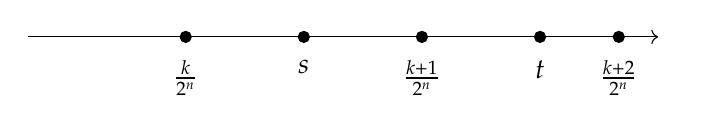
\begin{tikzpicture}
            % Draw number line
            \draw[->] (-2,0) -- (6,0) node[right] {};
        
            % Points on number line
            \draw[fill] (0,0) circle (2pt) node[below=5pt] {\(\frac{k}{2^{n}}\)};
            \draw[fill] (1.5,0) circle (2pt) node[below=5pt] {\(s\)};
            \draw[fill] (3,0) circle (2pt) node[below=5pt] {\(\frac{k+1}{2^{n}}\)};
            \draw[fill] (4.5,0) circle (2pt) node[below=5pt] {\(t\)};
            \draw[fill] (5.5,0) circle (2pt) node[below=5pt] {\(\frac{k+2}{2^{n}}\)};
        \end{tikzpicture}
    \end{figure}
    Then applying that $\omega \not \in A_{n}$, we have that:
    \begin{align*}
        |W_t - W_s| &\leq |W_t - W_{t \land (k+1)/2^{n}}| + |W_{t \land (k+1)/2^{n}} - W_{k/2^n}| + |W_s - W_{k/2^{n}}| \\
        &\leq 3 \cdot \sqrt{2n} 2^{-n/2} \leq 3\sqrt{2 |t-s|\log(1/|t-s|)} 
    \end{align*}
    The function $\sqrt{x\log(1/x)}$ is increasing in a neighborhood of 0 , so as long as $|t-s| \leq 2^{-(N+2)}$ and $\delta$ is below that increasing threshold, we are good. This shows that as long as $\delta \leq 2^{-(N+2)}$, we have:
    \begin{align*}
        \sup_{s, t \in [0,1], 0 < |t-s| < \delta} \frac{|W_t - W_s|}{\sqrt{\delta \log(1/\delta)}} &\leq 3\sqrt{2}
    \end{align*}
    Which completes the proof.

    \subsection*{Problem 7.4}
    Supose that $\alpha > 1/2$ and $W_t$ is a brownian motion. Show that the event
    \begin{align*}
        A = \qty{\exists t \in [0,1] : W \text{ is Holder continuous of order $\alpha$ at $t$}}
    \end{align*}
    has probability 0.

    Fix $N$ be so large that $N(\alpha - 1/2) > 1$, and define:
    \begin{align*}
        A_{M,h} = \qty{\exists s \in [0,1] : |W_t - W_s| \leq M|t-s|^\alpha, |t-s| \leq h } \\
        B_n = \qty{\exists k \leq 2n : \bigwedge_{i=1}^N |W_{(k+i)/n} - W_{(k+i-1)/n}| \leq \frac{2 N^\alpha M}{n^\alpha} }
    \end{align*} 
    I show that for $n \geq \frac{N}{h}$, $A_{M,h} \subset B_n$. This is becaus for $k$ the largest integer with $k/n \leq s$, $\qty|\frac{k+i}{n} - s| \leq \frac{N}{n} \leq h$. Then,
    \begin{align*}
        \qty|W_{(k+i)/n} - W_{(k+i-1)/n}| &\leq |W_{(k+i)/n} - W_s| + |W_s - W_{(k+i-1)/n}| \\
        &\leq \frac{N^\alpha M}{n^\alpha} + \frac{N^\alpha M}{n^\alpha} = \frac{2 N^\alpha M}{n^\alpha}
    \end{align*}
    Now, using independent increments, and that $P(|Z| \leq r) \leq 2r$ for standard normal $Z$,
    \begin{align*}
        P(B_n) \leq 2n P\qty(|W_{1/n}| \leq \frac{2 N^\alpha M}{n^\alpha})^N = 2n P\qty(|Z| \leq \frac{2 N^\alpha M}{n^{\alpha - 1/2}})^N \leq 2n \frac{4 N^{\alpha N} M^{N}}{n^{N(\alpha - 1/2)}} = C n^{-\beta}
    \end{align*}
    for some $\beta > 0$ by our choice of $N$ (recall $N(\alpha - 1/2) > 1$). This shows that 
    \begin{align*}
        P(A_{M,h}) \leq \limsup_{n \to \infty} P(B_n) = 0.
    \end{align*} This implies that the probability that there exists $s \leq 1$ such that
    \begin{align*}
        \limsup_{h \to 0} \frac{|W_{s+h} - W_s|}{|h|^\alpha} \leq M
    \end{align*}
    is zero, which shows that in fact, $W_t$ is not Holder continuous of order $\alpha$ at any $s \in [0,1]$.

    \subsection*{Problem 7.8}
    Let $H_\gamma(A)$ be the Hausdorff measure of order $\gamma$. Many books (see, for example, Stein \& Shakarchi Book 3) have shown that $H_\gamma(A)$ is a true measure on the borel subsets of $\R$. Using this, we know that if $C_n \downarrow C$, then $\lim_{n \to \infty} H_\gamma(C_n) = H_\gamma(C)$. Let $C_n$ be the $n$th level of the cantor set. $C_n$ is a union of $2^n$ intervals of length $3^{-n}$. So letting $\delta$ be arbitrary, choose $n$ so that $3^{-n} < \delta$. The order $\gamma = \log 2 / \log 3$ length of $C_n$ is $2^n \cdot 3^{- \gamma n} = 1$. This shows that 
    \begin{align*}
        \lim_{\delta \to 0} \qty[\inf\qty{\sum_{i=1}^\infty [b_i-a_i]^\gamma : A \subset \bigcup_{i=1}^\infty [a_i,b_i], \sup_i |b_i-a_i| \leq \delta}] \leq 1
    \end{align*} in particular it is finite. So the Hausdorff dimension of $C$ is at most $\log 2 / \log 3$. Now, suppose that it were less than $\log 2 / \log 3$. Then $H_\gamma(C_n) \leq M$ for some $\gamma = \log 2 / \log 3 - \ve$ and all $n \geq N$, by the limit argument. Since if $[a,b]$ is an interval covered by $\bigcup_i [a_i,b_i]$, all of which have length $\leq |b-a|$, we must have 
    \begin{align*}
        \sum_i |b_i-a_i| \geq |b-a|
    \end{align*} by union bound and the regular lebesgue measure. But then I claim that:
    \begin{align*}
        \sum_i |b_i-a_i|^{\gamma} \geq |b-a|^{\gamma}
    \end{align*} 
    This follows since:
    \begin{align*}
        \sum_i \qty(\frac{|b_i-a_i|}{|b-a|})^{\gamma} \geq \sum_i \frac{|b_i-a_i|}{|b-a|} \geq 1
    \end{align*}
    The first inequality is true as $\frac{|b_i-a_i|}{|b-a|} \leq 1$ and $x^\gamma \geq x$ for $x \leq 1$. So in particular, $H_\gamma([a,b]) \geq |a-b|^\gamma$. By disjointness, $H_\gamma(C_n) \geq 2^n \cdot 3^{-n \gamma} = 3^{n \ve}$. Sending $n \to \infty$ yields a contradiction.

    With that done, we prove exercise 7.7.
    \subsubsection*{Problem 7.7.}
    Let $W$ be a brownian motion and let $Z$ be the zero set $Z = \SET{t \in [0,1] : W_t = 0}$. 
    \begin{enumerate}
        \item Show there exists a constant $c$ not depending on $x$ or $\delta$ such that:
        \begin{align*}
            P(\exists s \leq \delta : W_s = -x) \leq ce^{-x^2/ 2\delta}
        \end{align*}
        \item Use the Markov Property of brownian motion to show that there exists a constant $c$ not depending on $s$ or $t$ such that:
        \begin{align*}
            P(Z \cap [s,t] \neq \emptyset) \leq c \qty (1 \wedge \sqrt{\frac{t-s}{t}})
        \end{align*}
    \end{enumerate}
    The first is a simple application of Doob's maximal inequality. Indeed, $P(\exists s \leq \delta : W_s = -x) \leq P(\sup_{s \leq \delta} |W_s| \geq |x|) \leq 2e^{-x^2/2\delta}$ per prop 3.15 in the book. 

    For the second, notice that $P(Z \cap [s,t] \neq \emptyset) = P(\exists \delta \leq t-s : W_{s + \delta} - W_s = -W_s)$. By what we proved above, and using that $W_{s + \delta} - W_s$ is a brownian motion independent of $\mathcal F_s$, we have:
    \begin{align*}
        P(\exists \delta \leq t-s : W_{s + \delta} - W_s = -W_s) &= E(P(\exists \delta \leq t-s : W_{s + \delta} - W_s = -W_s \mid \mathcal F_s)) \leq E(2e^{-W_s^2 / 2(t-s)})\\
    \end{align*}
    This equals:
    \begin{align*}
        \frac{2}{\sqrt{2 \pi s}} \int_{-\infty}^{\infty} e^{-x^2 / 2(t-s)} \cdot e^{-x^2 / 2s} dx = 2 \sqrt{\frac{t-s}{t}} 
    \end{align*}
    Since probabilities are less than 1, we immediately get $P(Z \cap [s,t] \neq \emptyset) \leq 2\qty(1 \land \sqrt{\frac{t-s}{t}})$.

    Let $C_n$ be the (random) collection of intervals $[i/2^n, (i+1)/2^n]$ that intersect $Z$. Then $\# C_n$ is a real-valued random variable of our brownian motion. By 7.7 and lineararity of expectation, we have:
    \begin{align*}
        E[\# C_n] = \sum_{i=0}^{2^n - 1} P(Z \cap [i/2^n, (i+1)/2^n] \neq \emptyset) \leq 2\sum_{i=0}^{2^n - 1} \frac{1}{\sqrt{i}} \leq \int_0^{2^n} \frac{2}{\sqrt{x}} = 4 \cdot 2^{n/2}
    \end{align*}
    The cover $C_n$ of $Z$ has Hausdorff $\gamma$ measure:
    \begin{align*}
        \sum_{[i/2^n, (i+1)/2^n] \in C_n} |2^{-n}|^{\gamma} = 2^{-n \gamma} \# C_n
    \end{align*}
    Thus, for each $\delta$ you can find an $n$ with $2^{-n} < \delta$, also with:
    \begin{align*}
        E(2^{-n \gamma} \# C_n) \leq 4 \cdot 2^{-n \gamma} \cdot 2^{n/2}
    \end{align*}
    We have found a sequence of covers $C_n$ of $Z$ with diameter shrinking to 0 so that its $1/2$ Hausdorff measure is finite almost surely. Taking a limit, with probability 1, the Hausdorff $1/2$ measure of all the $C_n$'s bounded by 4 almost surely. As the quantity $\inf \SET{\sum_{i=1}^\infty [b_i-a_i]^\gamma : A \subset \cup_{i=1}^\infty [a_i,b_i], \; \sup_i [b_i-a_i] \leq \delta }$ is increasing in $\delta$, the limit as $\delta \to 0$ exists (possibly infinite), and equals the same among any sequence of $\delta$'s going to 0. This concludes the proof that $H_{1/2}(Z)$ is finite a.s., meaning that the Hausdorff dimension of $Z$ is at most $1/2$. 
\end{document}